\documentclass{article}

\usepackage{polski}
\usepackage{amsmath, array}
\usepackage{graphicx}
\usepackage{float}
\usepackage{subfig}
\usepackage{multirow}
\usepackage{enumitem}

\title{Laboratorium 11}
\author{\textbf{Łukasz Wala}\\
    \textit{AGH, Wydział Informatyki, Elektroniki i Telekomunikacji} \\
    \textit{Teoria Współbieżności 2022/23}}
\date{Kraków, \today}

\begin{document}
\maketitle

\section{Treść zadania}

Napisz program w dowolnym języku, który:
\begin{enumerate}
    \item Wyznacza relację niezależności $I$
    \item Wyznacza ślad $[w]$ względem relacji $I$
    \item Wyznacza postać normalną Foaty FNF$([w])$ śladu $[w]$
    \item Wyznacza graf zależności dla słowa $w$
    \item Wyznacza postać normalną Foaty na podstawie grafu
\end{enumerate}

\section{Implementacja}

Rozwiązanie zostało napisane w języku Python. W kodzie zamieszczone są komentarze
opisujące działanie programu:

\begin{verbatim}
    class DependencyGraph:
    def __init__(self, word, indep_rel):
        self.word = word
        self.indep_rel = indep_rel
        self.edges = self.calc_edges()
        self.remove_transitive_edges()
        self.dot = self.to_dot("g")

    def calc_edges(self):
        # tworzone są krawędzie grafu w postaci listy sąsiedztwa
        edges = [[] for _ in self.word]
        for i, letter in enumerate(self.word[:-1]):
            for j, other_letter in enumerate(self.word[i+1: ], i+1):
                if (letter, other_letter) not in self.indep_rel:
                    edges[i].append(j)
        
        return edges

    def remove_transitive_edges(self):
        # usuwane są krawędzie przechodnie
        to_remove = set()
        for i in range(len(self.word)):
            for j in self.edges[i]:
                for k in list(set(self.edges[i]) & set(self.edges[j])):
                    to_remove.add((i, k))

        for a, b in list(to_remove):
            self.edges[a].remove(b)

    def to_dot(self, name):
        # zapisywanie grafu w formacie dot
        dot = f"digraph {name} {'{'}\n"
        for i in range(len(self.word)):
            for j in self.edges[i]:
                dot += f"  {i} -> {j}\n"
        
        for i, letter in enumerate(self.word):
            dot += f"  {i}[label={letter}]\n" 

        return dot + "}\n"
    

class Problem:
    def __init__(self, alphabet, indep_rel, word):
        self.alphabet = alphabet
        self.indep_rel = indep_rel | {(b, a) for a, b in indep_rel}
        self.dep_rel = self.calc_dep_rel()
        self.word = word
        self.trace = self.calc_trace()
        self.normal_form = self.calc_normal_form()
        self.graph = self.calc_graph()

    def calc_dep_rel(self):
        # od iloczynu kartezjańskiego alfabetu z samym sobą
        # odejmowany jest self.dep_re w sensie zbiorów
        return {(a,b) for a in alphabet for b in alphabet} - self.indep_rel

    def calc_trace(self):
        # dla każdego słowa w zbiorze dotychczasowym zbiorze śladów
        # stwórz nowy zbiór, gdzie w każdym słowie zamienione są sąsiednie litery,
        # jeżeli należą do relacji niezależności
        # operacja jest powtarzana do momentu, 
        # kiedy nowy zbiór oraz stary zbiór są takie same
        word_set = {self.word}

        while True:
            next_set = set(word_set)
            for w in word_set:
                for i in range(len(w) - 1):
                    start, c1, c2, end = w[:i], w[i], w[i + 1], w[min(i + 2, len(w)):]
                    if (c1, c2) in self.indep_rel:
                        next_set.add(start + c2 + c1 + end)

            if word_set == next_set:
                break
            word_set = next_set

        return word_set

    def calc_normal_form(self):
        # tutaj zaimplementowany jest algorytm obliczaznia formy nornalnej Foaty
        # używany w laboratorium 10
        stacks = {letter: [] for letter in self.alphabet}
        for letter in reversed(self.word):
            stacks[letter].append(letter)
            for other_letter in self.alphabet - {letter}:
                if (letter, other_letter) in self.dep_rel:
                    stacks[other_letter].append(None)

        normal_form = []
        while any(stacks.values()):
            top_letters = [s[-1] for s in stacks.values() if len(s) and s[-1] is not None]
            for letter in top_letters:
                stacks[letter].pop()
                for other_letter in self.alphabet - {letter}:
                    if (letter, other_letter) in self.dep_rel:
                        stacks[other_letter].pop()
            
            normal_form.append(top_letters)

        return "".join([f"({''.join(sorted(i))})" for i in normal_form])

    def calc_graph(self):
        # tworzony jest graf zależności
        return DependencyGraph(self.word, self.indep_rel)

    def get_results(self):
        print(f"D = {self.dep_rel}")
        print(f"trace([{self.word}]) = {self.trace}")
        print(f"FNF([{self.word}]) = {self.normal_form}")
        print(f"Dependency graph for [{word}]:")
        print(self.graph.dot)


if __name__ == "__main__":
    alphabet = {"a", "b", "c", "d"}
    indep_rel = {("a", "d"), ("d", "a"), ("b", "c"), ("c", "b")}
    word = "baadcb"

    print("PROBLEM 1:")
    problem = Problem(alphabet, indep_rel, word)
    problem.get_results()


    alphabet = {"a", "b", "c", "d", "e", "f"}
    indep_rel = {("a", "d"), ("d", "a"), ("b", "e"), ("e", "b"), \
        ("c", "d"), ("d", "c"), ("c", "f"), ("f", "c")}
    word = "acdcfbbe"
    print("\nPROBLEM 2:")
    problem = Problem(alphabet, indep_rel, word)
    problem.get_results()
\end{verbatim}

Dla przykładów podanych w kodzie powyżej program zwraca następujące rezultaty:

\begin{verbatim}
PROBLEM 1:
D = {('a', 'b'), ('b', 'd'), ('b', 'b'), ('a', 'a'), 
    ('b', 'a'), ('c', 'c'), ('d', 'b'), ('d', 'd'), 
    ('d', 'c'), ('c', 'd'), ('c', 'a'), ('a', 'c')}
trace([baadcb]) = {'bdaabc', 'badacb', 'bdaacb', 'badabc', 'baadcb', 'baadbc'}
FNF([baadcb]) = (b)(ad)(a)(bc)
Dependency graph for [baadcb]:
digraph g {
    0 -> 1
    0 -> 3
    1 -> 2
    2 -> 4
    2 -> 5
    3 -> 4
    3 -> 5
    0[label=b]
    1[label=a]
    2[label=a]
    3[label=d]
    4[label=c]
    5[label=b]
}

PROBLEM 2:
D = {('b', 'c'), ('f', 'a'), ('b', 'f'), ('b', 'd'), ('a', 'b'), 
    ('c', 'c'), ('c', 'e'), ('e', 'c'), ('f', 'b'), ('e', 'f'), 
    ('e', 'd'), ('e', 'e'), ('b', 'a'), ('d', 'b'), ('c', 'a'), 
    ('a', 'c'), ('e', 'a'), ('b', 'b'), ('a', 'f'), ('a', 'e'), 
    ('c', 'b'), ('f', 'd'), ('f', 'f'), ('f', 'e'), ('a', 'a'), 
    ('d', 'd'), ('d', 'f'), ('d', 'e')}
trace([acdcfbbe]) = {'dacfcbbe', 'acdcfbbe', 'adcfcbbe', 
    'adcfcebb', 'adccfbbe', 'accdfbeb', 'adfccbbe', 'adcfcbeb', 
    'accdfebb', 'dacfcebb', 'dacfcbeb', 'daccfebb', 'dafccbeb', 
    'acdcfbeb', 'adfccbeb', 'dafccebb', 'acdfcbbe', 'adccfbeb', 
    'acdfcebb', 'acdcfebb', 'dafccbbe', 'accdfbbe', 'acdfcbeb', 
    'daccfbbe', 'adccfebb', 'adfccebb', 'daccfbeb'}
FNF([acdcfbbe]) = (ad)(cf)(c)(be)(b)
Dependency graph for [acdcfbbe]:
digraph g {
    0 -> 1
    0 -> 4
    1 -> 3
    2 -> 4
    3 -> 5
    3 -> 7
    4 -> 5
    4 -> 7
    5 -> 6
    0[label=a]
    1[label=c]
    2[label=d]
    3[label=c]
    4[label=f]
    5[label=b]
    6[label=b]
    7[label=e]
}
\end{verbatim}

Grafy wygenerowane przez program wyglądają następująco:

\begin{figure}[H]
    \centering
    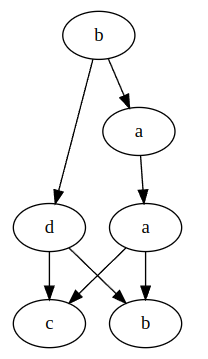
\includegraphics[width=0.4\textwidth]{graph_1.png}
    \caption{graf zależności Diekerta dla problemu 1}
\end{figure}

\begin{figure}[H]
    \centering
    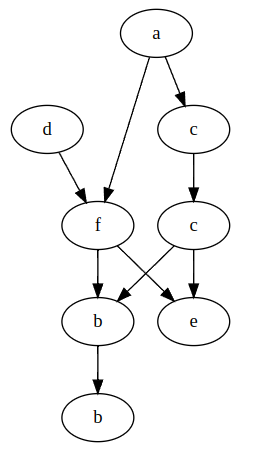
\includegraphics[width=0.4\textwidth]{graph_2.png}
    \caption{graf zależności Diekerta dla problemu 2}
\end{figure}

Wyniki, jak i uzyskane grafy zgadzają się z ręcznie otrzymanymi wynikami z poprzedniego
sprawozdania z laboratorium 10, co może sugerować poprawność działa programu.

\section{Wnioski}
Problem znalezienia zbioru relacji zależności oraz niezależności, śladu dla pewnego
ciągu akcji czy grafu zależności można zautomatyzować, używając prostych algorytmów. 

\section{Bibliografia}

\begin{enumerate}
    \item G. Rozenberg, A. Salomaa - \textit{Handbook of Formal Languages}
\end{enumerate}

\end{document}